\chapter{Project Monitoring}\label{project monitoring}

\section{Code Statistics}

\begin{figure}[H]

The actual \nameref{project_stages} are recognizable on the GitHub code frequency chart as well. In Elaboration and Construction most commits have been done while in the Transition phase the graph flattens out.

  \centering
  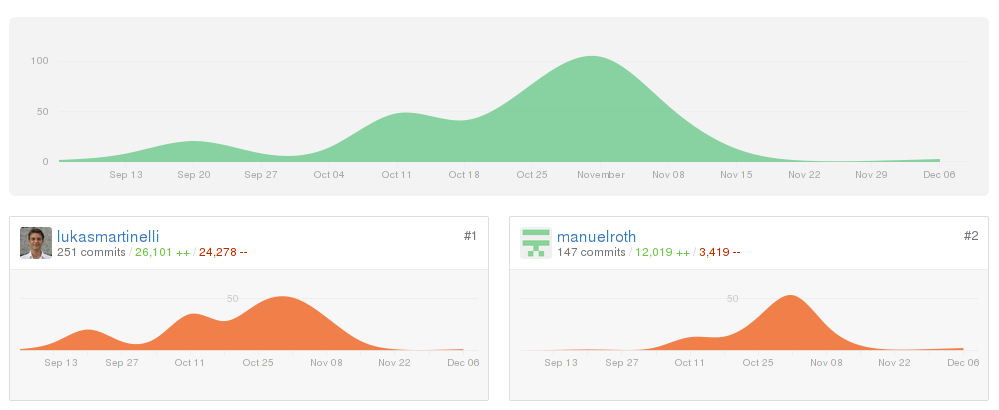
\includegraphics[width=1\textwidth]{images/github_commits.png}
  \caption{Commit frequency}
\end{figure}

\section{Estimated Time vs Actual Time}

Our estimations were too optimistic. Due to the extensive
training period required to get started in a GIS environment
the actual time was more than originally estimated.


\begin{table}[H]
\centering
    \begin{tabular}{lll}
    \textbf{Sprint}        & \textbf{Actual} & \textbf{Estimated} \\
     \hline
    Inception 1    & 20     & 16        \\
    Inception 2    & 42     & 55        \\
    Elaboration 1  & 48     & 50        \\
    Elaboration 2  & 121    & 102       \\
    Construction 1 & 152    & 106         \\
    Construction 2 & 48     & 53        \\
    Transition     & 61 & 98        \\
    \hline
    \textbf{Total}          & 493 & 480 \\
    \end{tabular}
    \caption{Estimated vs actual time for different sprints}
\end{table}
\newpage

\section{Time per Person}

Both contributors invested about the same amount of time.

\begin{table}[H]
\centering
    \begin{tabular}{llll}
    \textbf{Sprint}  & \textbf{Lukas Martinelli} & \textbf{Manuel Roth} & \textbf{Total} \\
    \hline
    Inception 1    & 11               & 9           & 20    \\
    Inception 2    & 22               & 21          & 43    \\
    Elaboration 1  & 25               & 23          & 48    \\
    Elaboration 2  & 56               & 65          & 121   \\
    Construction 1 & 77               & 75          & 152   \\
    Construction 2 & 27               & 21          & 48    \\
    Transition     & 28               & 33          & 61    \\
    \hline
    \textbf{Total}          & 245              & 248         & 493   \\
    \end{tabular}
    \caption{Time for each contributor for sprints}
\end{table}